\newpage

\section{Using existing EMF projects in eMoflon}
\visHeader

This chapter contains stepwise instructions on how to use existing \mbox{EMF}/Ecore projects with an eMoflon project specified using the visual syntax via EA.
We will present an example of an existing metamodel which must be integrated with eMoflon before, for example, its transformation using SDMs can be
specified. The basic workflow for using an existing EMF project in eMoflon is described in the following and may of course be similarly applied to a metamodel
specified in the textual syntax via MOSL. 

We will begin by implementing a small subset of the \texttt{Ecore -> GenModel} transformation, where \texttt{GenModel} is part of the EMF/Ecore standard. The
\emph{GenModel} for a given Ecore model can be viewed as a \emph{wrapper} that contains additional generation-specific Java code details. These details are
separated from the Ecore model to keep it free of such ``low-level'' information and settings.

\section{Modelling relevant aspects in EA}
\genHeader

The first step is to load an existing metamodel into EA. A complete and automatic import of existing Ecore files in EA is currently not possible and therefore,
\emph{relevant parts} of the existing metamodel (\texttt{GenModel}) have to be modelled manually. Although this might sound frightening (especially for
large, complex metamodels), the emphasis here on \emph{relevant} indicates that only elements that are needed for the transformation have to be present in
EA, where more can be added iteratively as the transformation grows. 

If you find this section challenging or unclear, refer to Part II: Ecore for a detailed review of metamodel construction.

\begin{stepbystep}

\item Open Eclipse and create a new metamodel project named \texttt{Ecore\-To\-Gen\-Model}, do not select the \texttt{Add Demo Specification}
option in the project wizard window.

\item A new specifications folder with the project name should have been loaded into the workspace.

\item Double-click the generated \texttt{Ecore\-To\-Gen\-Model.eap} file to open your project in EA. 
Explore the project browser and make note of the packages already present in EA under \texttt{eMoflon Languages}, especially \texttt{Ecore} which we shall use in this transformation.

\item Select the root note \texttt{My Working Set} and create a new package named \texttt{Gen\-Model\-Language}. 

\item Add a new Ecore diagram and model the elements as depicted in \Cref{fig_gMM}. You'll need to create the three EClasses on
the left, but \texttt{Ecore::EPackage} and \texttt{Ecore::EClass} are to be drag-and-dropped and pasted as links from the project browser. 

\vspace{0.5cm}

\begin{figure}[htbp]
\begin{center}  
	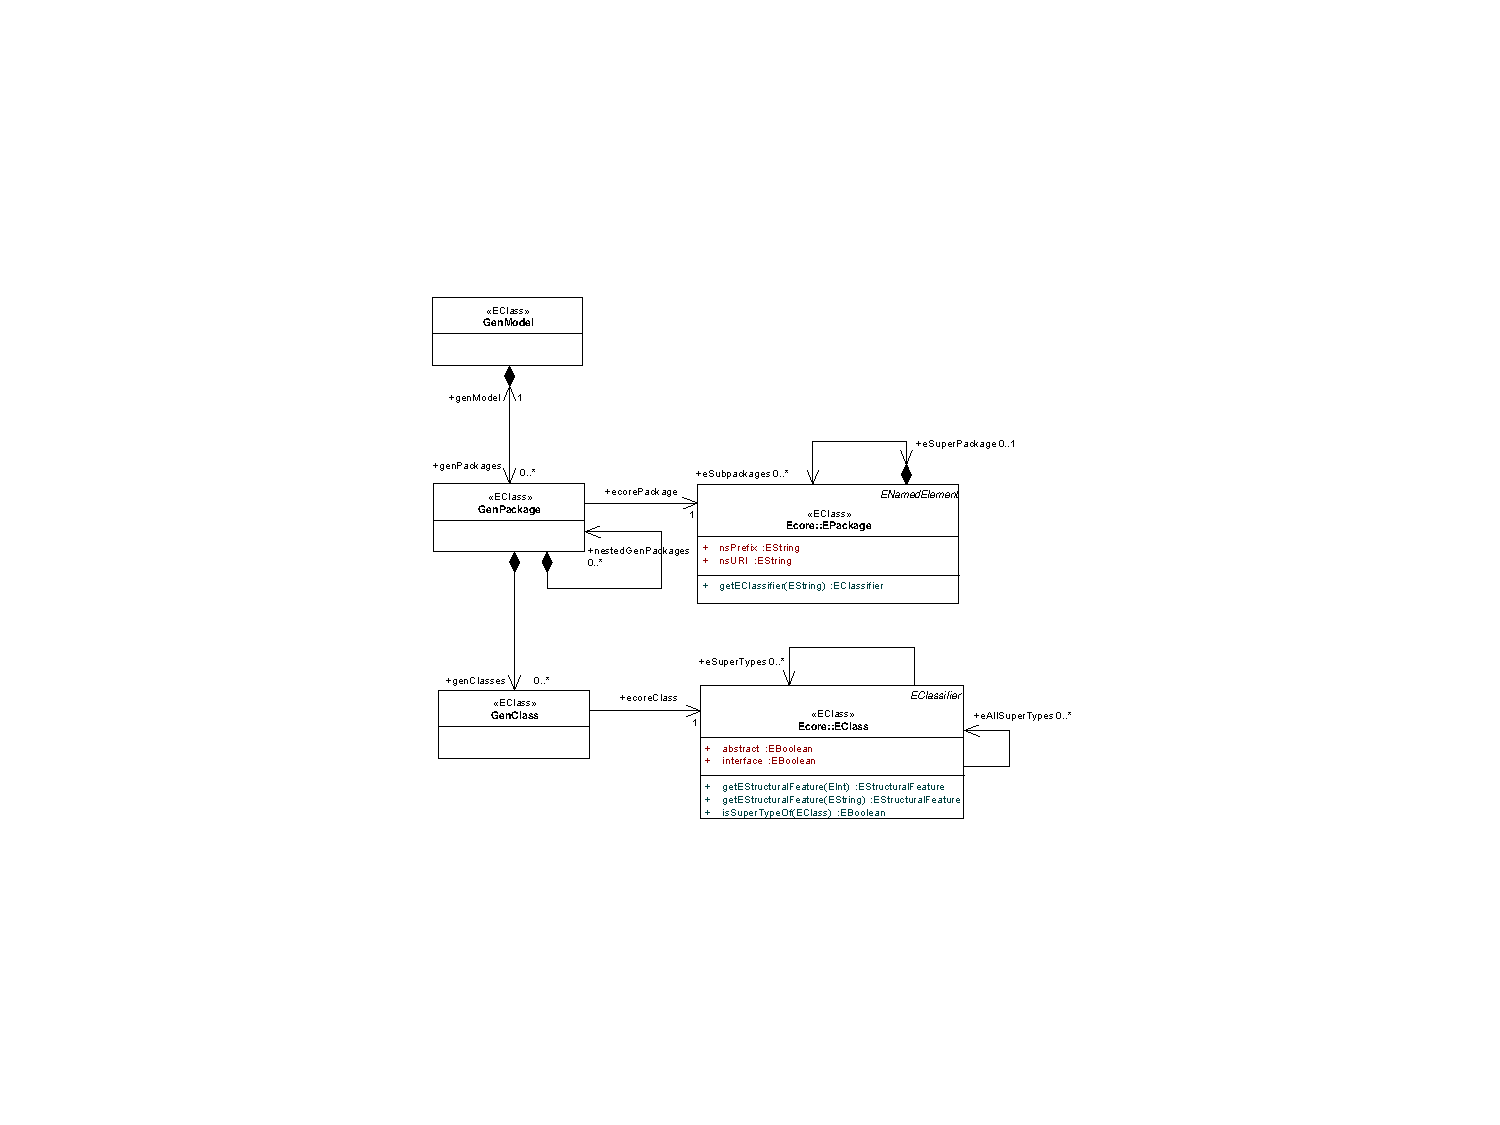
\includegraphics[width=\textwidth]{../../org.moflon.doc.handbook.05_miscellaneous/3_existingEMF/emfImages/CDGenmodel.pdf}
	\caption{Metamodel of \texttt{GenModel}}  
\label{fig_gMM}
\end{center}
\end{figure} 

\vspace{0.5cm}

\item Please note that the actual \texttt{GenModel} metamodel contains many more elements, but this subset is sufficient for our
task.
Although this subset can be incomplete, it must be correct and not contradict the actual \texttt{GenModel} metamodel in any way!

\item Navigate to the project browser again and create another package named \texttt{Ecore2GenModel}.  
This will contain the \texttt{Transformer} class; Create and complete its Ecore diagram as depicted in \Cref{fig_e2gm}.

\item Carefully double-click each method to create and implement their SDMs as depicted in \Cref{fig_pack2g,fig_transf}.
\end{stepbystep}

\newpage

\vspace*{2cm}

\begin{figure}[htbp]
	\begin{center}  
	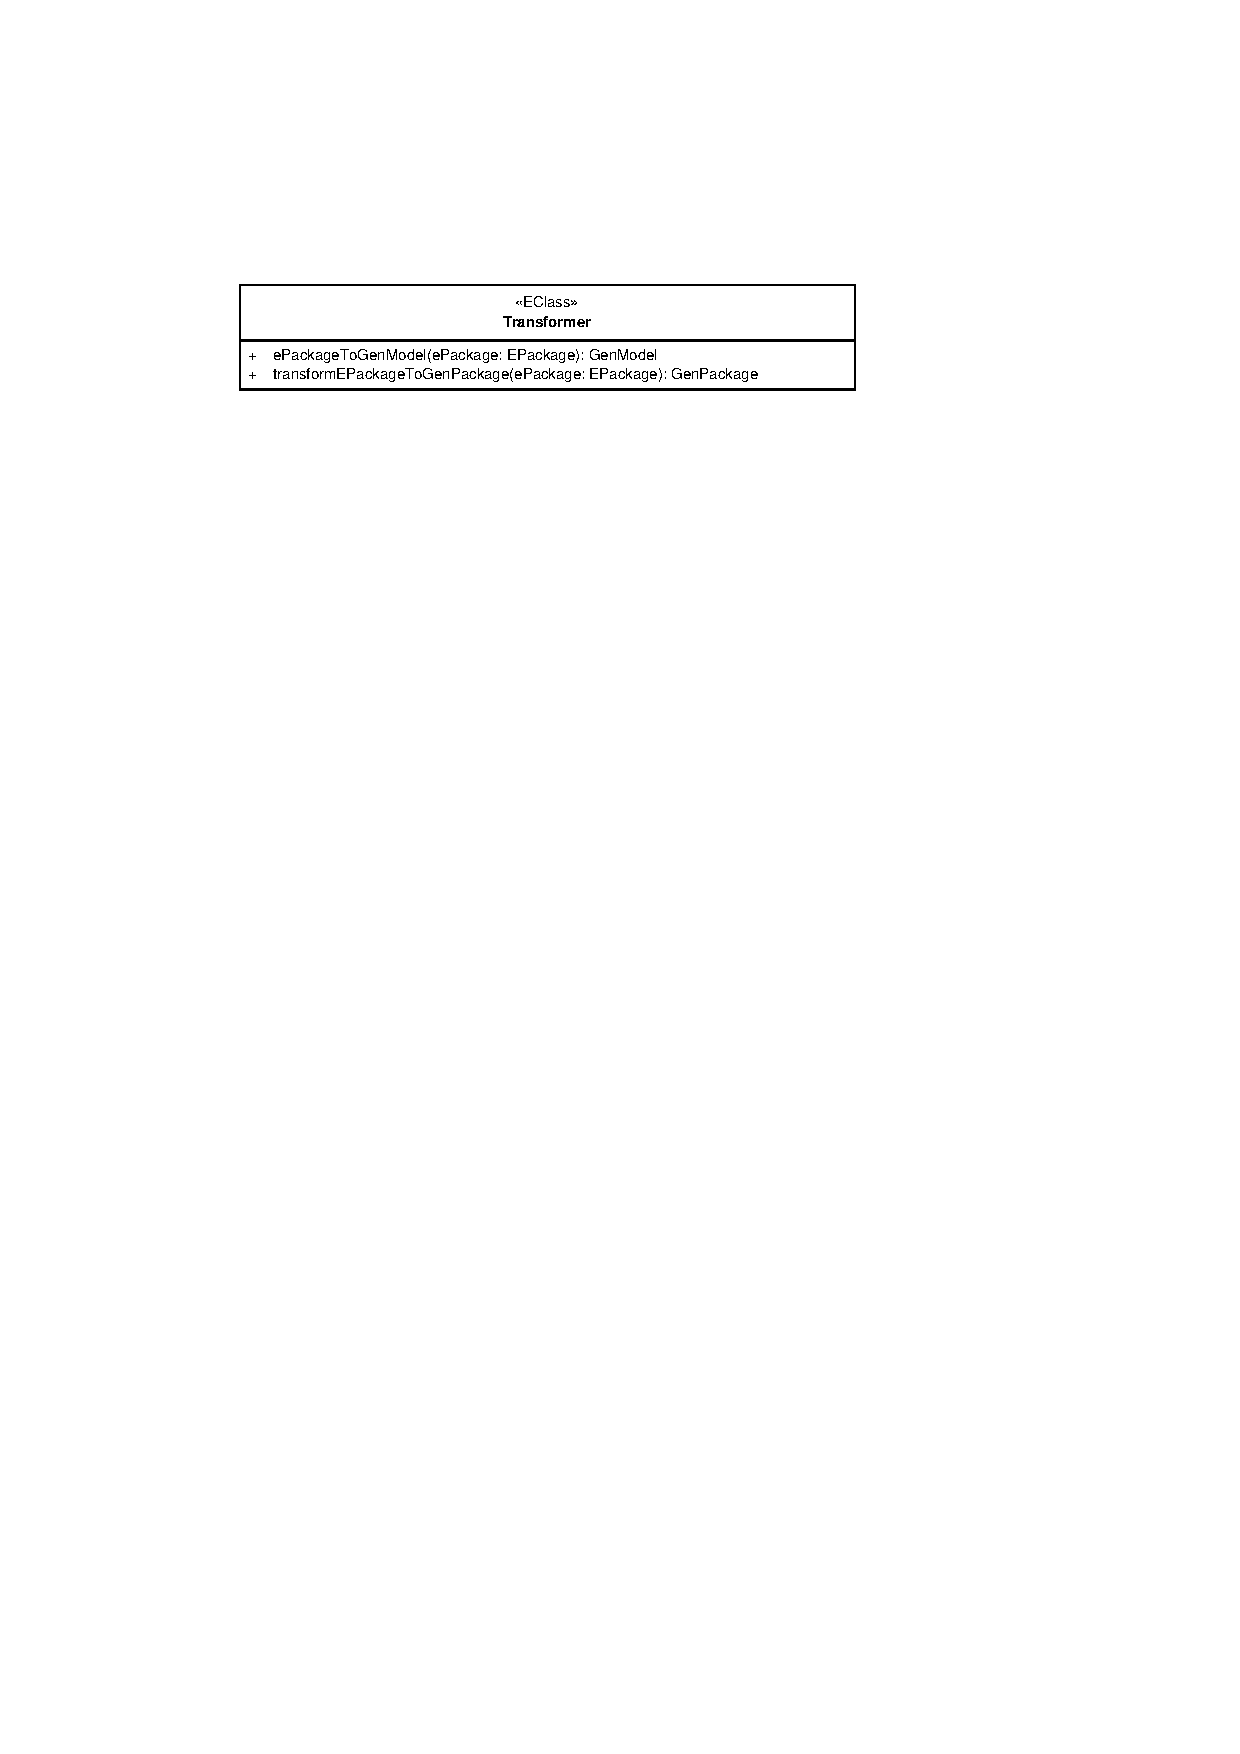
\includegraphics[width=0.7\textwidth]{../../org.moflon.doc.handbook.05_miscellaneous/3_existingEMF/emfImages/CDTransformer.pdf}
	\caption{Methods in \texttt{Transformer}}  
	\label{fig_e2gm}
	\end{center}
\end{figure} 

\vspace{1cm}

\begin{figure}[htbp]
\begin{center}  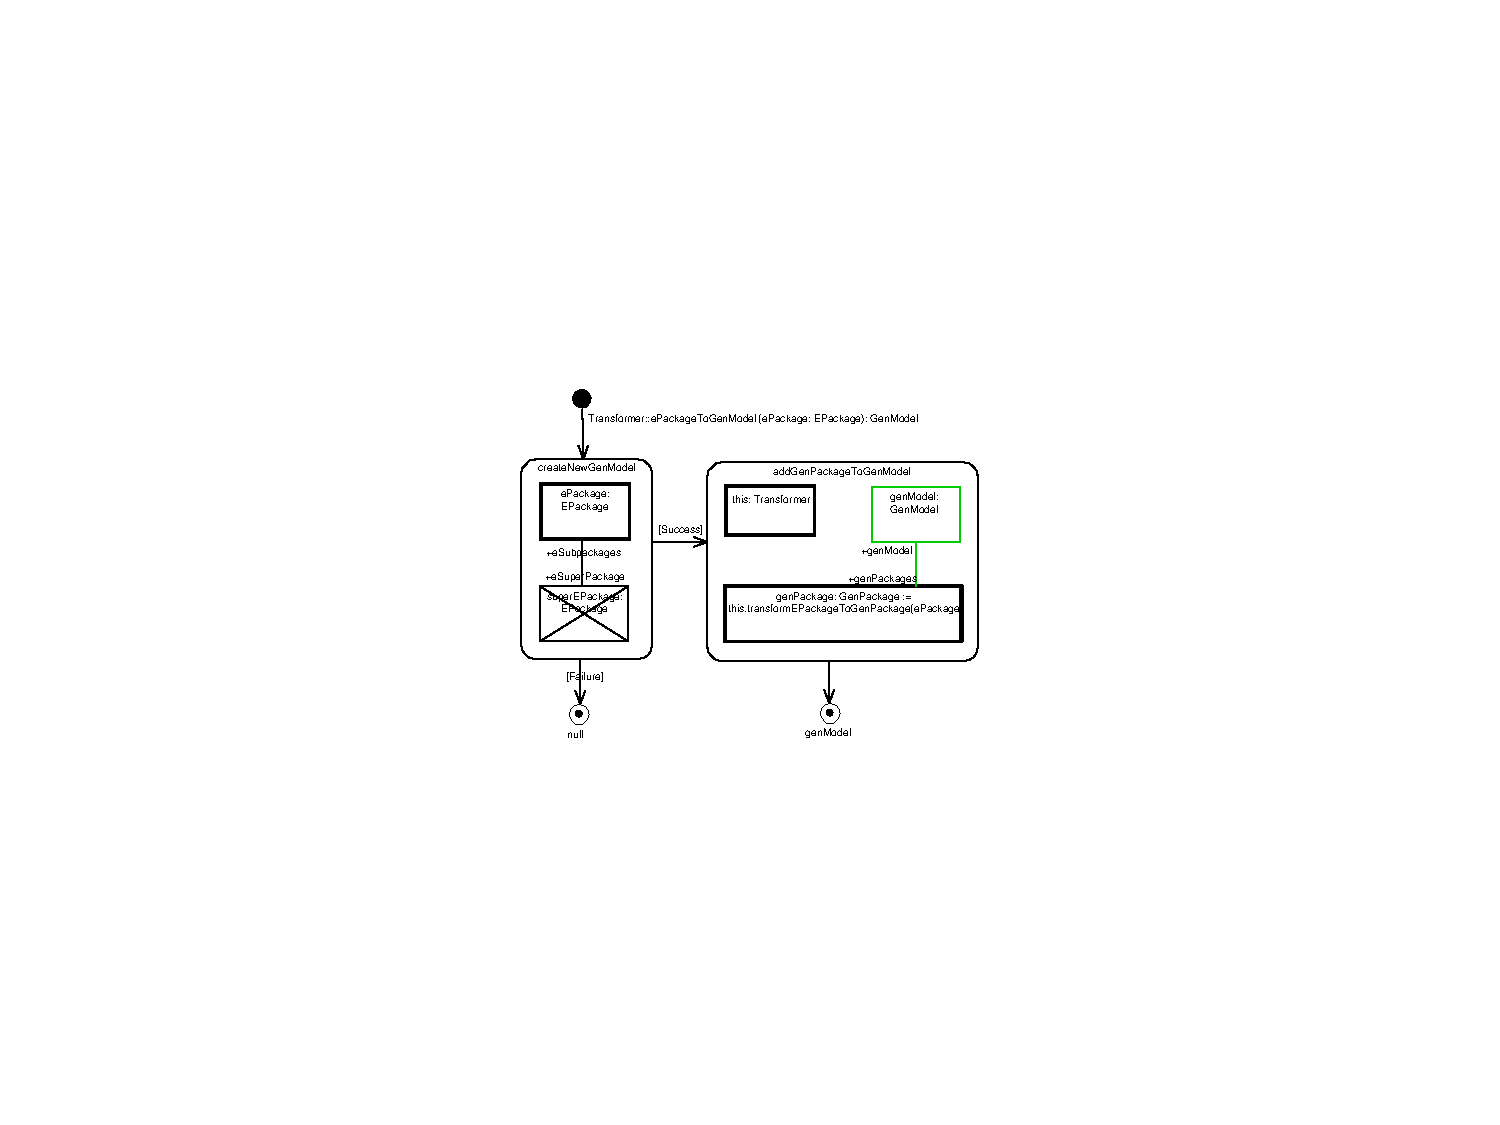
\includegraphics[width=0.8\textwidth]{../../org.moflon.doc.handbook.05_miscellaneous/3_existingEMF/emfImages/SDMePackageToGenModel.pdf}
        \caption{Main method for \texttt{EPackage} to \texttt{GenModel} transformation}  
  \label{fig_pack2g}
\end{center}
\end{figure} 

\begin{figure}[htbp]
\begin{center}  
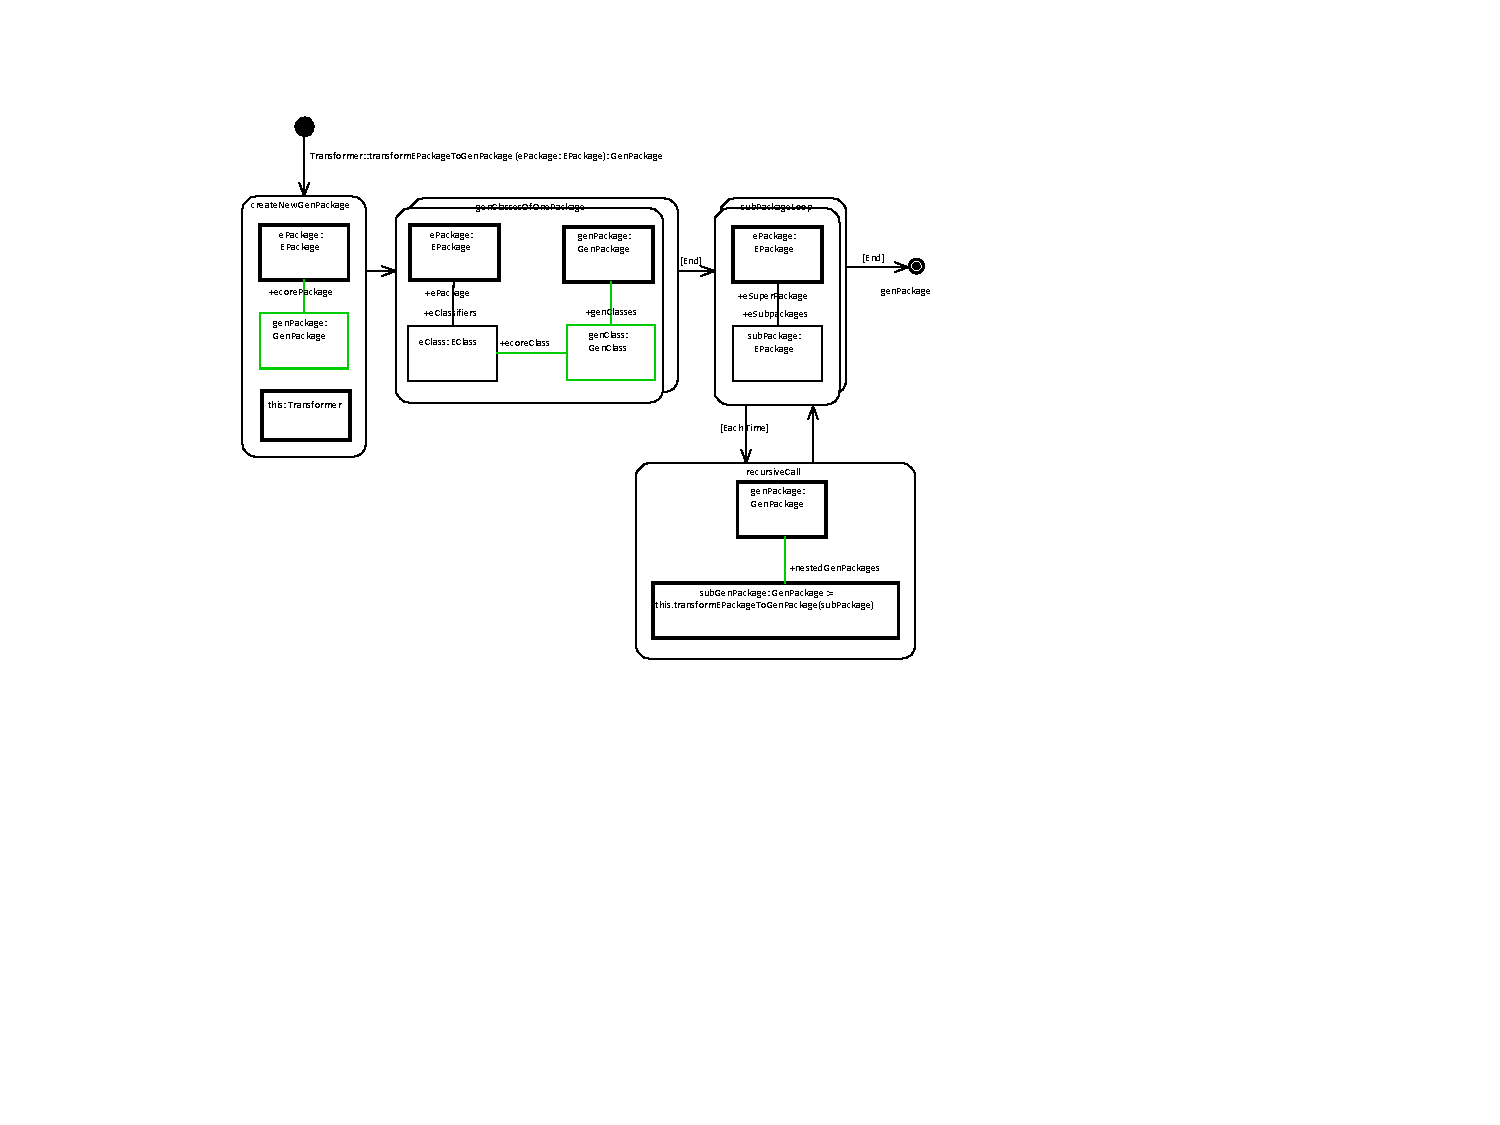
\includegraphics[width=1.1\textwidth]{../../org.moflon.doc.handbook.05_miscellaneous/3_existingEMF/emfImages/SDMtransformEpackageToGenPackage.pdf}
\caption{Helper function to transform all \texttt{EPackages} to \texttt{GenPackages}}  
\label{fig_transf}
\end{center}
\end{figure} 



\newpage

\subsection{Configuration for code generation in Eclipse}
\genHeader

Since there is already generated code for the existing \texttt{GenModel} metamodel (provided via the Eclipse plugin), we do \emph{not} want to export our
incomplete subset of \texttt{GenModel} from EA. Instead, we need to configure Eclipse to access the elements specified in our partial metamodel from the
complete metamodel.

\begin{enumerate}

\item[$\blacktriangleright$] In EA, right-click your \texttt{GenModelLanguage} package and select ``Properties\ldots'' 

\item[$\blacktriangleright$] Navigate to ``Properties/Moflon'' in the dialogue window and update the tagged \texttt{Moflon::Export} value to \texttt{false}
(Fig.~\ref{fig_customNS}).

\vspace{0.5cm}

\begin{figure}[htb]
\begin{center}  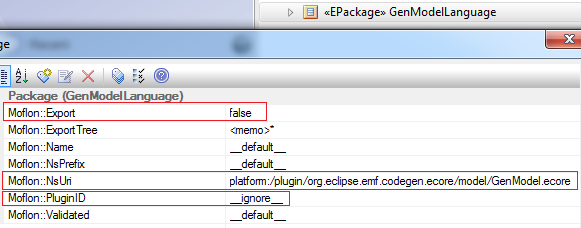
\includegraphics[width=\textwidth]{ea_genModelExportFalse}
  \caption{Update the \texttt{GenModel} export option and create custom tags}  
  \label{fig_customNS}
\end{center}
\end{figure}

\newpage

\item[$\blacktriangleright$] Next we have to set the ``real'' name and URI of the project to be used in Eclipse so that the relevant references are exported
properly. In the same window, create new tagged values \texttt{Moflon::CustomNsPrefix} and \texttt{Moflon::CustomNsUri}.

\item[$\blacktriangleright$] Set their values to \texttt{genmodel} and \texttt{http://\-www.\-eclipse.\-org/\-emf/\-2002/\-GenModel} respectively, as shown in
Fig.~\ref{fig_customNS}. These values can be determined by inspecting the corresponding values in the existing .ecore file (i.e.,~the existing metamodel).

\item[$\blacktriangleright$] Validate and export all projects as usual to your Eclipse workspace, and update the metamodel project by pressing \texttt{F5} in
the package explorer.

\item[$\blacktriangleright$] In order to simplify setting the required dependencies for code generation,  convert the generated Eclipse project
\texttt{Ecore2GenModel} to a \emph{plug-in project} by right-clicking the project and selecting ``Configure/Convert to Plug-in Projects...''

\item[$\blacktriangleright$] Right-click \texttt{Ecore2GenModel} once more and navigate to ``Plug-in Tools/Open Manifest.'' The plug-in manager should have
opened in the editor with a series of tabs at the bottom for each option.

\item[$\blacktriangleright$] Switch to the \texttt{Dependencies} tab. Press \texttt{Add} and enter \texttt{org.\-eclipse.\-emf.\-codegen.\-ecore}. This plug-in
includes both the \texttt{Ecore} and \texttt{Gen\-Mod\-el} libraries we require.

\end{enumerate}

Although we have already specified the name and URI of the existing project (in this example, \texttt{GenModel}) as tagged project values, we now have to tell
eMoflon where to find the correct implementation (generated code) of the existing project.

\begin{enumerate}
  
\item[$\blacktriangleright$] Expand the \texttt{Ecore2GenModel} project folder and open the \texttt{mof\-lon.\-prop\-er\-ties.\-xmi} file tree. Right-click the
properties container, and create a new \texttt{Add\-it\-ion\-al Dep\-en\-den\-cies} child. Double click the element to open its properties tab below the
editor, and as shown in Fig.~\ref{eclipse:addDepChild}, update its \texttt{Value} to:\\
\end{enumerate}

\vspace{-1cm}
{\small \ttfamily  platform:/plugin/org.eclipse.emf.codegen.ecore/model/GenModel.ecore} \\
\vspace{-0.5cm}

\begin{figure}[htbp]
\begin{centering}
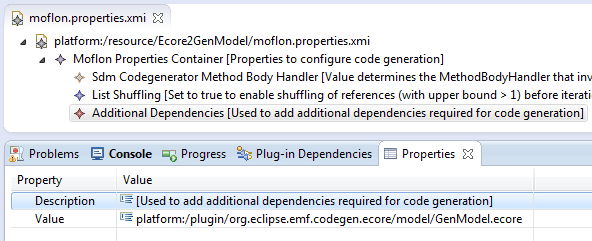
\includegraphics[width=\textwidth]{eclipse_additDepProps}
  \caption{Setting properties for the correct implementation code}  
  \label{eclipse:addDepChild}
\end{centering}
\end{figure} 

\begin{enumerate}

\item[$\blacktriangleright$] Similarly, add a second \texttt{Additional Used Gen Packages} child and set its value to: \\
\end{enumerate}

\vspace{-1cm}
{\small \ttfamily platform:\-/\-plugin/\-org.\-eclipse.\-emf.\-codegen.\-ecore/\-model/\-GenModel.\-genmodel}

\newpage
Finally, to compenstate for some cases where our naming conventions were violated, analogously add the following mapping as corrections:

\begin{enumerate}
\item[$\blacktriangleright$] Add an \emph{import mapping} child for correct generation of the required import, setting the key as \texttt{genmodel} (as
depicted in Fig.~\ref{eclipse:impMapValues}) and value to: \\
{\small \ttfamily \hspace*{1.5cm} org.\-eclipse.\-emf.\-codegen.\-ecore.\-genmodel}

\vspace{0.5cm}

\begin{figure}[htbp]
\begin{centering}
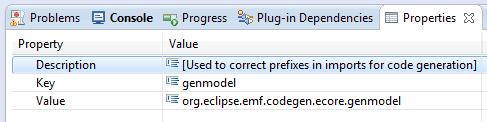
\includegraphics[width=0.9\textwidth]{eclipse_importMappingValues}
  \caption{Mapping properties from our metamodel to the existing \texttt{GenModel}}  
  \label{eclipse:impMapValues}
\end{centering}
\end{figure} 

\item [$\blacktriangleright$] Finally, add a \emph{factory mapping} to ensure that \texttt{GenModelFactory} is used as the factory for creating elements in the
transformation instead of \texttt{Genmodel\-Factory}, which would be the default convention. Set its key as \texttt{genmodel}, and its value to:
{\small \ttfamily GenModelFactory}.

\item [$\blacktriangleright$] Your completed \texttt{moflon.properties.xmi} file should now closely resemble Fig.~\ref{eclipse:finalPropTree}. Refresh your
workspace one more time to generate code for the project and ensure that the transformation behaves as expected via a JUnit test.

\newpage

\vspace*{2cm}

\begin{figure}[htbp]
\begin{centering}
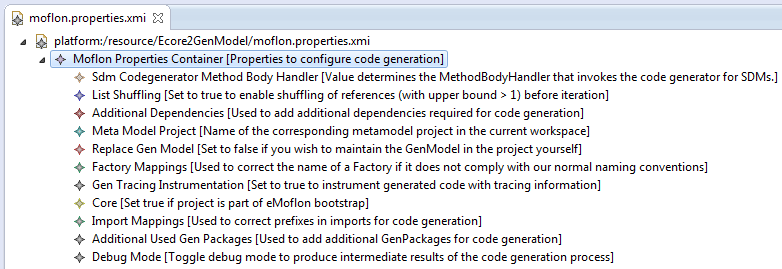
\includegraphics[width=\textwidth]{eclipse_finalPropTree}
  \caption{Additional properties for code generation}  
  \label{eclipse:finalPropTree}
\end{centering}
\end{figure} 

\end{enumerate}

